%Thema im Praktikum soll dynamische Programmierung werden
%\chapter{Vorlesung}
\chapter{Minimal aufspannende Bäume MST}	%Werden 2 Algorithmen machen
\paragraph{Eingabe}
\[ G=(V,E)~~E~\text{ungerichtet}~~(u,v)\in E \Rightarrow (v,u)\in E\text{ mögliche Notation } \{ u,v \} \]
$ w:E\rightarrow \mathbb{R}$
\paragraph{Gesucht}
\[ \text{Baum }T \subseteq E\]
\[ G_T=(V,T) \text{zusammenhängend (zykelfrei)} \]
\[ w(T) = \sum_{e\in T} w(e) \text{minimal} \]
\begin{figure}[H]
\centering
\begin{subfigure}[H]{0.3\textwidth}
	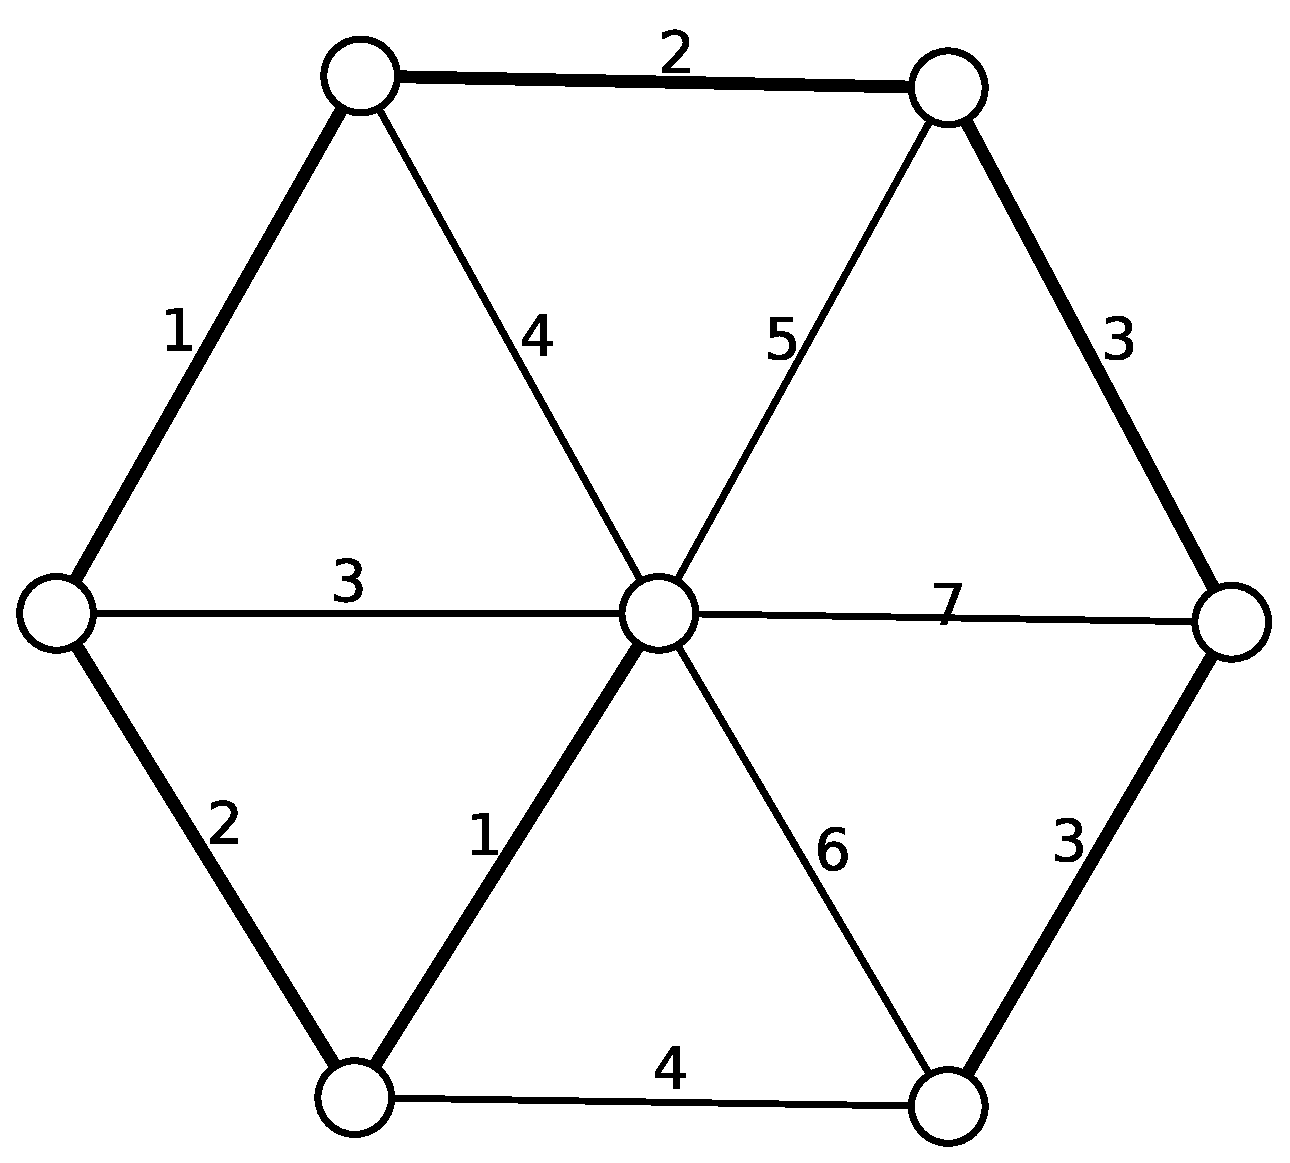
\includegraphics[width=\linewidth]{19/Grafik/Spannbaum}
	\caption{Beispiel für einen Spannbaum in einem Graphen}
	\label{fig:Spannbaum}
\end{subfigure}
\begin{subfigure}[H]{0.3\textwidth}
	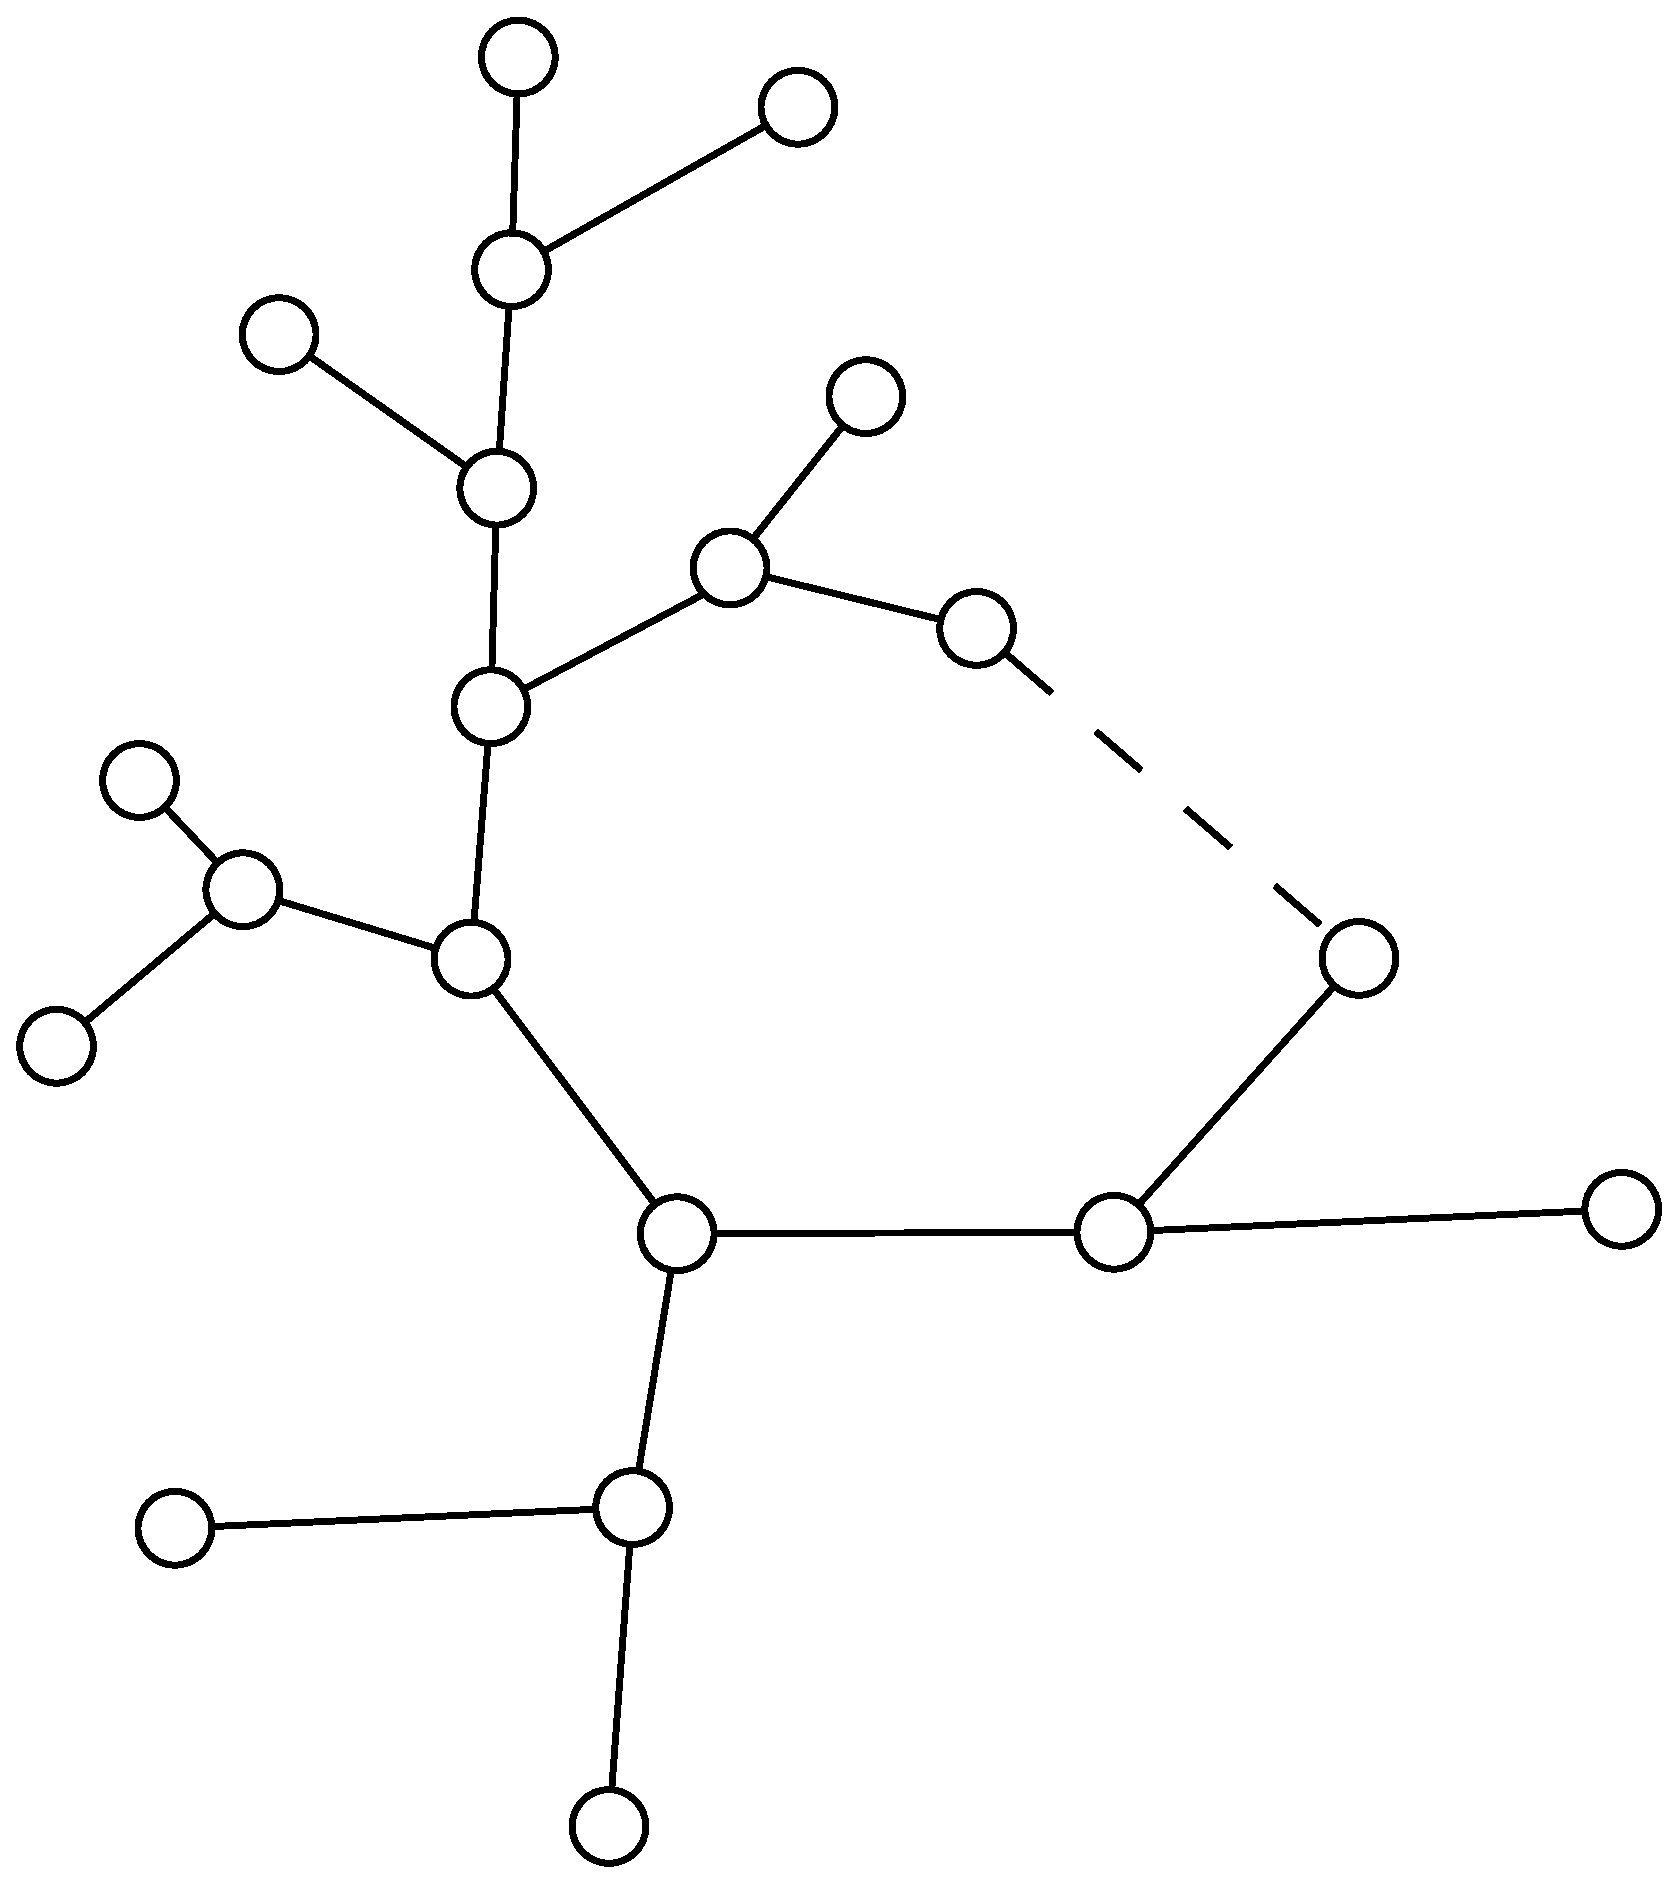
\includegraphics[width=\linewidth]{19/Grafik/SpannbaumBeispiel2}
	\caption{Beispiel für einen Spannbaum}
	\label{fig:Spannbaum2}
\end{subfigure}
\begin{subfigure}[H]{0.3\textwidth}
	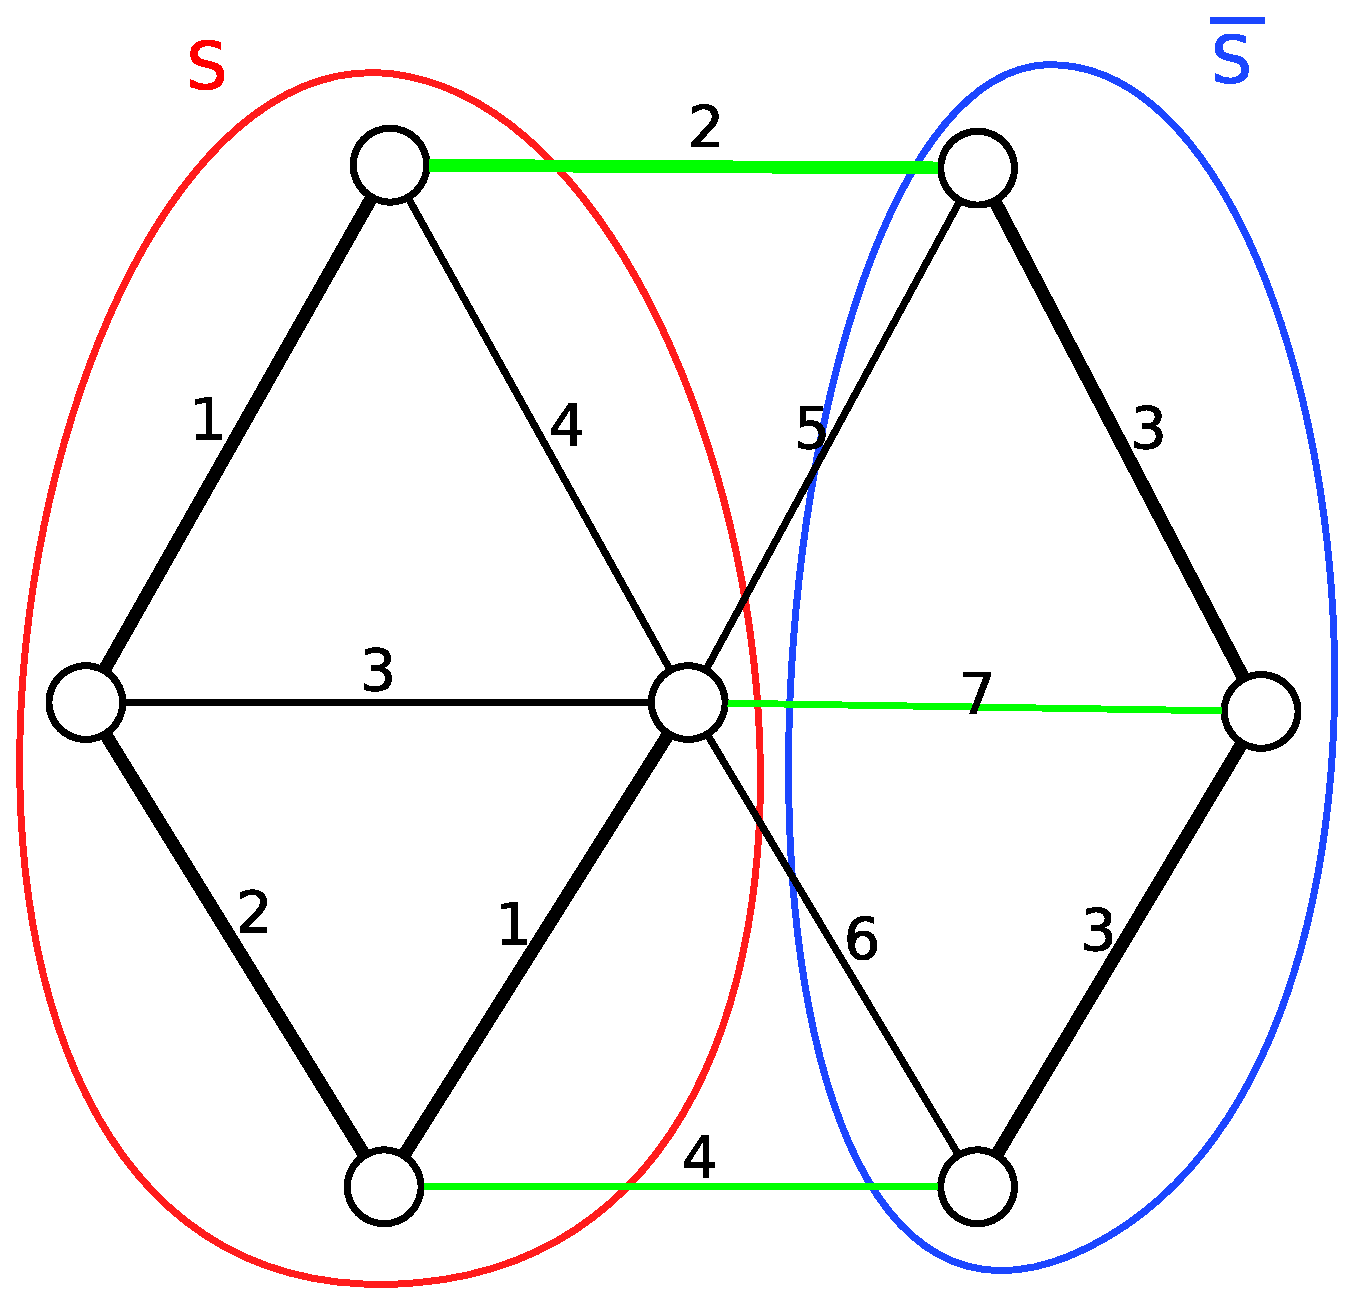
\includegraphics[width=\linewidth]{19/Grafik/Schnittlemma1}
	\caption{\textcolor{green}{Grün} markiert sind alle Kanten, die von \textcolor{red}{$S$} nach \textcolor{blue}{$\overline{S}$} verlaufen. Wähle die Kante mit dem kleinsten Gewicht, also 2, aus.}
	\label{fig:Spannbaum3}
\end{subfigure}
\end{figure}

%Bild1 und 2
\paragraph{Frage} $|T|= $?
\paragraph{Antwort} $|T| = |V|-1$
\section{Greedy-Algorithmen zur Lösung des MST-Problems:}
Starte mit $T=\emptyset$, nehme sukzessive Kanten zu $T$ hinzu, so dass nach $|V|-1$ Schritten der gesuchte MST entstanden ist. 
Dabei benötigen wir ein Kriterium, das sicherstellt, dass gewählte Kanten zur Gesamtlösung dazugehören.
\section{Schnitt-Lemma:}
Betrachte eine Aufteilung (Schnitt) der Knotenmenge $V$ in $V$ und $\overline{S} = V\setminus S$ \\und Kanten $(u,v) \in E \cap S\times \overline{S}$\\
Sei $e \in E \cap S \times \overline{S}$ mit $w(e) \leq w(e') ~\forall ~e' \in E \cap S\times \overline{S}$ dann gibt es einen MST mit $e \in$ MST
\subsection{Beweis für das Schnitt-Lemma}
\begin{figure}[h]
\centering
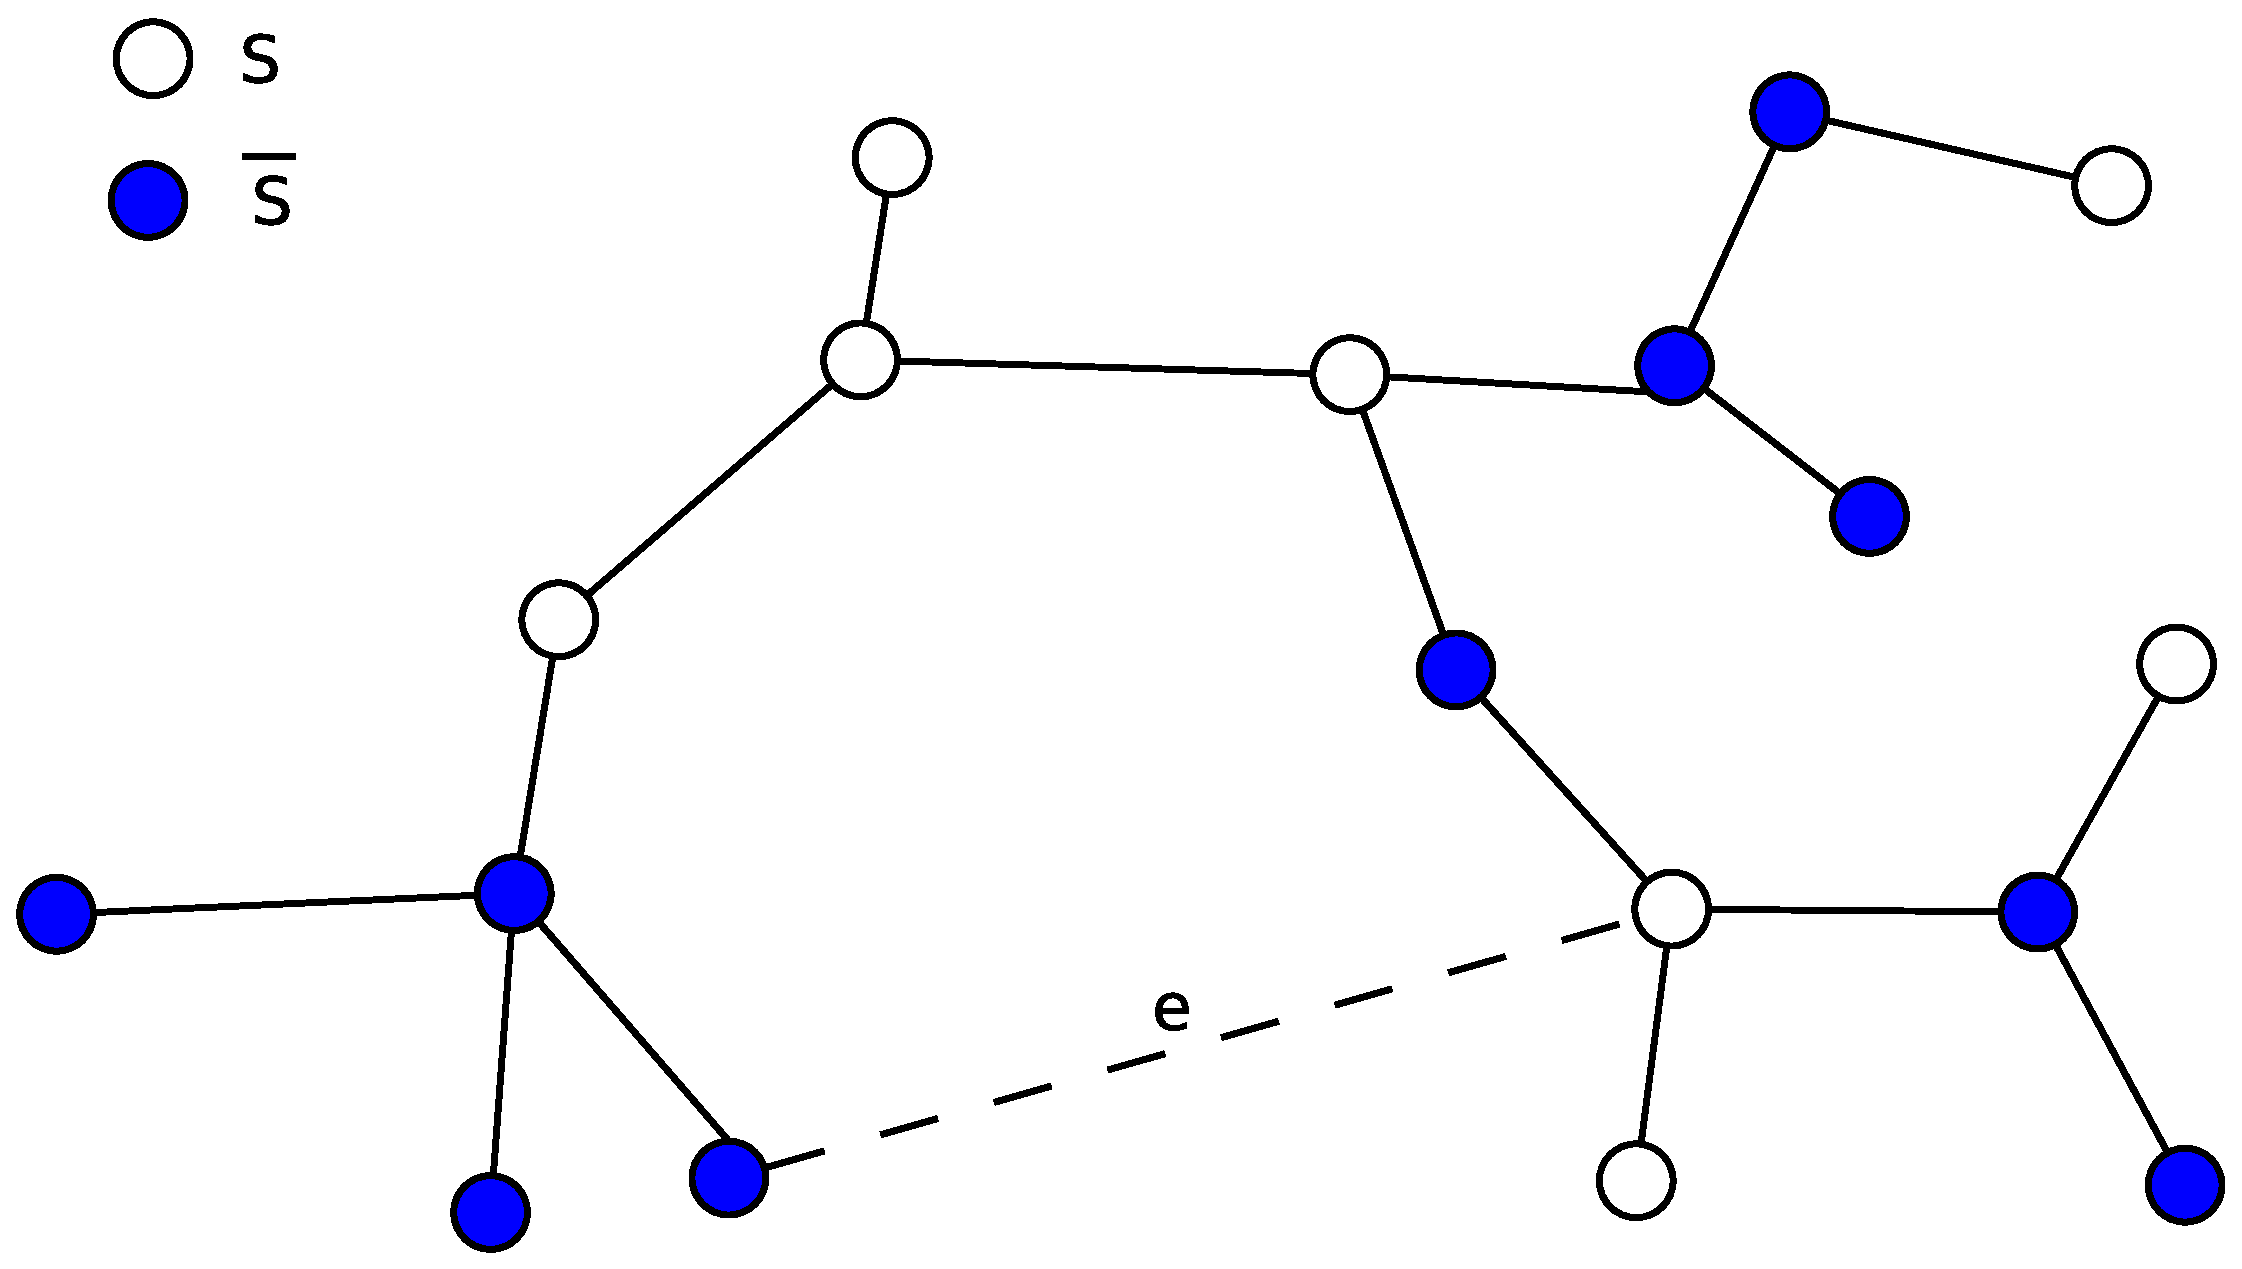
\includegraphics[width=0.5\linewidth]{19/Grafik/SpannbaumBeweis}
\caption{}
\label{fig:SpannbaumBeweis}
\end{figure}

Sei e eine "`sichere"' Kante aus dem Schnitt-Lemma.\\
o.B.d.A. $u\in S$ und $v \in \overline{S}$.\\
Es gibt eine Zykel in $T\cup \{e\}$ und darin eine Kante $e'\in S\times \overline{S}$ mit $w(e') \geq w(e)$.\\
Ersetze $T'=T\cup\{e\}\setminus\{ e' \}$\\
$w(T') \leq w(T) \Rightarrow w(T') = w(T)$ weil $T$ ein MST.
\begin{flushright}
	q.e.d.
\end{flushright}
\section{Algorithmus von Kruskal}
sortiere Kanten nach ihrem Gewicht aufsteigend\\
$T=\emptyset$\\

\begin{wrapfigure}{R}{0.5\linewidth}
	\vspace*{-80pt}
	\centering
	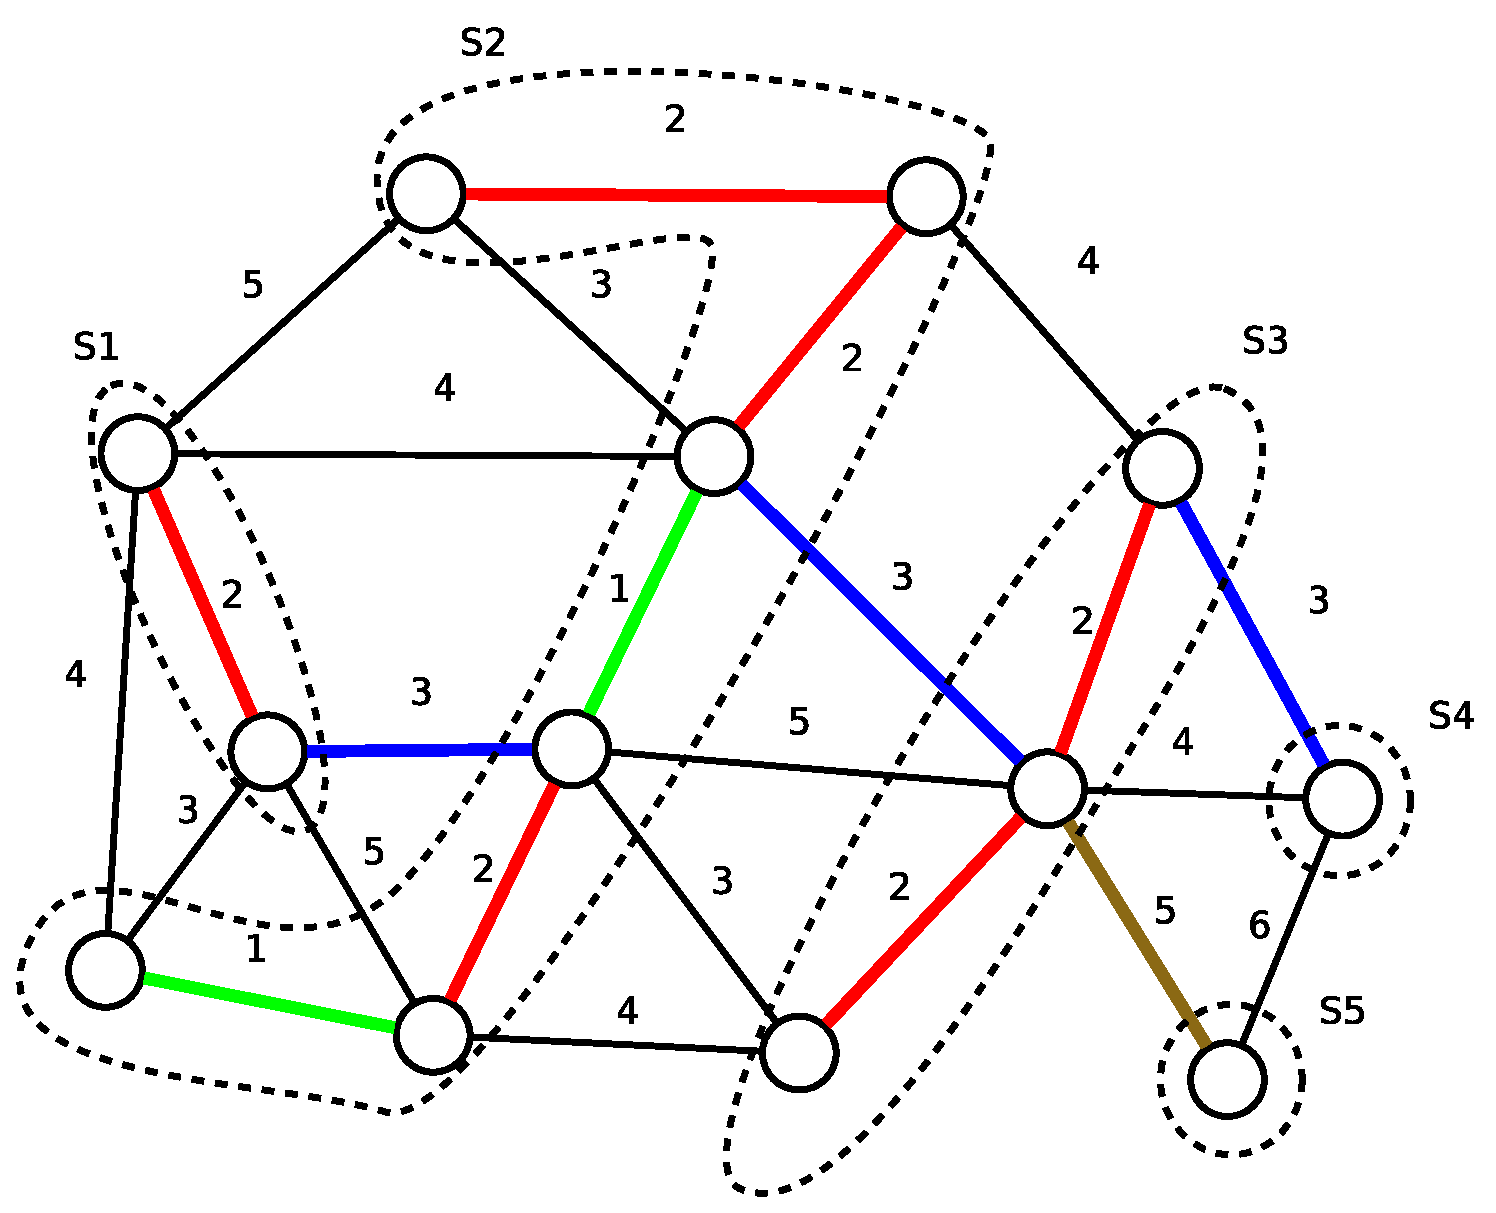
\includegraphics[width=\linewidth]{19/Grafik/SpannbaumBeispiel3}
	\caption{Reihenfolge grün$\rightarrow$rot$\rightarrow$blau$\rightarrow$braun}
	\label{fig:Beispiel3}
	\vspace{-500pt}
\end{wrapfigure}
\begin{lstlisting}
forall (u,v) /eIn E in sortierter Reihenfolge {
	if (find(u) == find(v)) continue;
	T = T$\cup${(u,v)};
	union(u,v);
}
\end{lstlisting}
\subsubsection{Effizienz von Kruskal}
\paragraph{Sortieren:} $\mathcal{O}(|E|\cdot\log|E|) = \mathcal{O}(|E|\log|V|)$\\
$2|E|$ viele find-Operationen $\mathcal{O}(1)$\\
$\underline{|V|-1}$ viele union-Operationen $\mathcal{O}(|V|)$ naiv\\
$\mathcal{O}(|E|\log|V|+|E|\cdot 1 + (|V|-1)|V|) =$\\ $\mathcal{O}(|E|\log|V|+$\sout{$|V|^2$}$)$\\
\subsubsection{Idee zum Aufbau einer Union-Find-Datnstruktur}
Jeder Knoten trägt eine Komponentennummer, die in einem Feld vermerkt ist. Die find-Operation ist durch einen Feld-Zugriff realisierbar. Um die union-Operation zu realisieren, verwalten wir die Knoten einer Komponente in einer einfach verketteten Liste und merken uns die Listenlänge. Wenn zwei Komponenten fusionieren, benennen wir die Komponente mit der kleineren Knotenzahl um, indem wir die zugehörige Liste durchlaufen und die Umbenennung im Feld vornehmen. Und die beiden betroffenen Listen müssen konkateniert werden.
\paragraph{Beobachtung:} Ein einzelner Knoten erfährt höchstens $\log|V|$ viele Umbenennungen seiner Komponentennummer, da sich bei jeder Umbenennung die Größe der Komponente zu der er gehört, verdoppelt.